\documentclass{beamer}
\usepackage[latin1]{inputenc}
\usepackage{color}
\usepackage[absolute,overlay]{textpos}
\usetheme{Warsaw}

\expandafter\def\expandafter\insertshorttitle\expandafter{%\insertshorttitle\hfill%
  \insertframenumber\,/\,\inserttotalframenumber}

\definecolor{red}{rgb}{1,0,0}
\title[TagFS]{A tag based filesystem}
\author{Catalina Macalet, Eugen Hristev, Mihai Dinu, Sorin Dumitru}
\institute{Politehnic University of Bucharest}
\date{Jan 12, 2010}
\begin{document}

\begin{frame}
  \titlepage
\end{frame}

\section{Introduction}
\begin{frame}{Table of contents}
    \begin{itemize}
        \item{Introduction}
        \item{Related work}
	\item{Architecture}
	\item{VFS \& TagFS Operations}
	\item{Implementation details}
	\item{Conclusions}
    \end{itemize}
\end{frame}

\begin{frame}{Introduction}
    \begin{itemize}
        \item{Looking for alternatives for the classic file system}
        \item{TagFS - tag based file system}
	\item{Tag files and browse files by tags}
        \item{Personalized content and user-friendly}
    \end{itemize}
\end{frame}

\begin{frame}{Related work}
    \begin{itemize}
        \item{TagFS: Bringing Semantic Metadata to the Filesystem}
	\begin{itemize}
		\item \url{http://www.eswc2006.org/poster-papers/FP31-Schenk.pdf}
	\end{itemize}
        \item{Nepomuk-KDE}
	\begin{itemize}
		\item \url{http://nepomuk.kde.org/}
	\end{itemize}
	\item{TaggedFrog}
	\begin{itemize}
		\item \url{http://lunarfrog.com/}
	\end{itemize}
    \end{itemize}
\end{frame}

\section{Architecture}
\begin{frame}{TagFS hierarchy}
\begin{itemize}
	\item {The filesystem hierarchy whill remain unchanged but files will have associated tags}
	\item{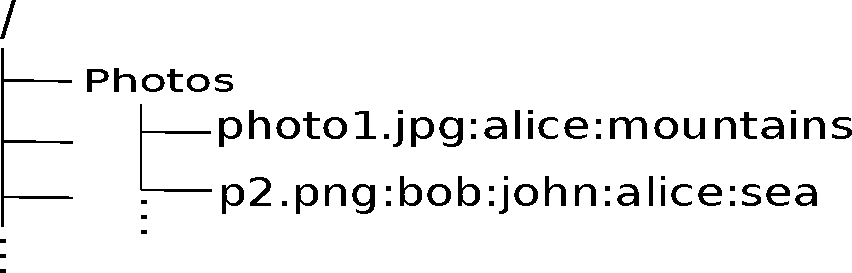
\includegraphics[scale=0.5]{figs/hierarchy.pdf}}
\end{itemize}
\end{frame}

\begin{frame}{TagFS architecture}
\begin{itemize} 
	\item {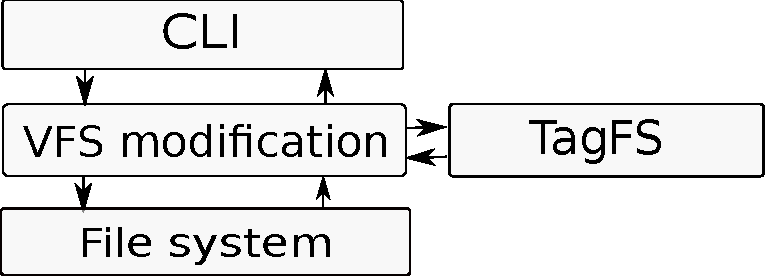
\includegraphics[scale=0.7]{figs/archall.pdf}}
\end{itemize}
\end{frame}

\begin{frame}{Database}
\begin{itemize} 
	\item{Multiple files mapped to a tag}
	\item {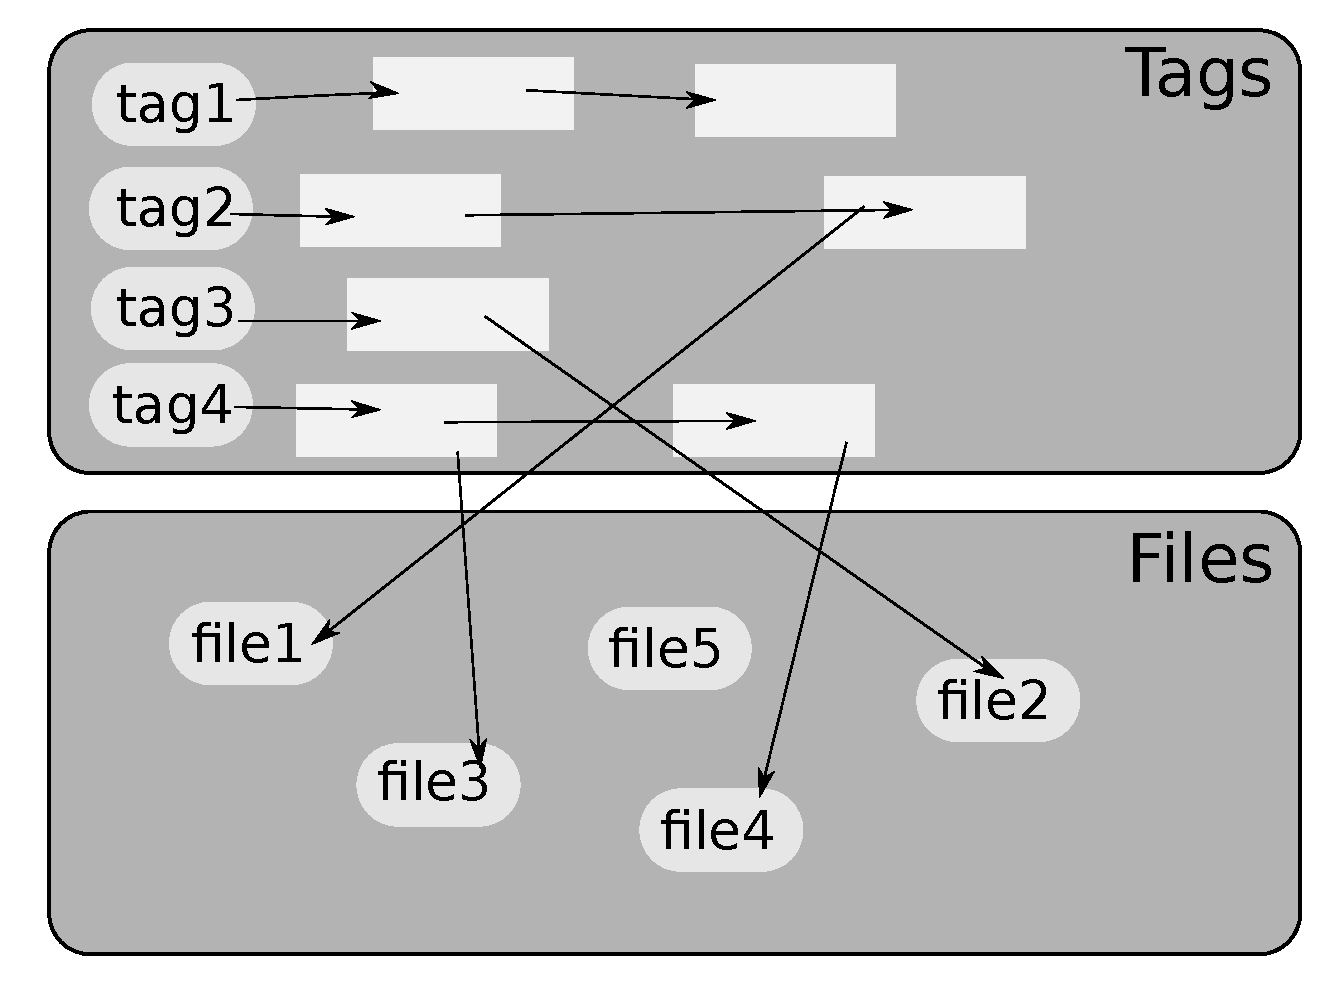
\includegraphics[scale=0.3]{figs/storage.pdf}}
\end{itemize}
\end{frame}

\section{VFS \& TagFS Operations}
\begin{frame}{VFS Operations}
    \begin{itemize}
        \item \textcolor{red}{touch filename:tag1:tag2:...}
            \begin{itemize}
                \item{create file with tags (add metadata in tagfs structure)}
                \item{vfs function: do$\_$sys$\_$open}
            \end{itemize}
        \item \textcolor{red}{mv}
            \begin{itemize}
                \item{move file (change metadata in tagfs structure)}
                \item{vfs function: rename}
            \end{itemize}
        \item \textcolor{red}{cp}
            \begin{itemize}
                \item{create a copy of file (add metadata in tagfs structure)}
                \item{vfs function: unlink}
            \end{itemize}
        \item \textcolor{red}{ls}
            \begin{itemize}
                \item{list files and associated tags, iterate through tagfs structure}
                \item{vfs function: getdents}
            \end{itemize}
    \end{itemize}
\end{frame}

\begin{frame}{TagFS Operations}
    \begin{itemize}
        \item {All use fcntl syscall}
        \item \textcolor{red}{ tag -l filename}
            \begin{itemize}
                \item{list tags associated with a file}
            \end{itemize}
        \item \textcolor{red}{ tag -a filename:tag1:tag2:...}
            \begin{itemize}
                \item{Add tag1, tag2,.. tags to file}
            \end{itemize}
        \item \textcolor{red}{ tag -d filename:tag1:tag2:...}
            \begin{itemize}
                \item{Remove tag1, tag2,... tags from file}
            \end{itemize}
    \end{itemize}
\end{frame}


\section{Implementation Details}
\begin{frame}{TO DO}
    \begin{itemize}
      \item{To Do...}
    \end{itemize}
\end{frame}


\section{Conclusions}
\begin{frame}{Conclusions}
    \begin{itemize}
        \item {Improvements:}
	\begin{itemize}
		\item{Lower external fragmentation of disk}
	\end{itemize}
        \item {A tag file system is a feasible solution now-a-days}
	\item {Some more stuff written here ~~~} 
    \end{itemize}
\end{frame}

\begin{frame}{Questions?}
    \begin{itemize}
	\item {Thank you !} 
    \end{itemize}
\end{frame}

\end{document}
